\documentclass[11pt]{article}

\usepackage{geometry}
\usepackage{fancyhdr}
\usepackage{graphicx}

\title{Adatbázisrendszerek I. Assigment}
\author{Orosz Péter - WO02D7}

\graphicspath{{./images/}}

\geometry{margin=3cm}

\pagestyle{fancy}
\setlength{\headheight}{15pt}
\fancyhead[R]{\thepage}
\fancyhead[L]{Adatbázisrendszerek I. Assignment - Orosz Péter - WO02D7}
\fancyfoot[C]{University of Miskolc}

\fancypagestyle{plain}{%
	\fancyhf{}%
	\fancyhead[R]{\thepage}%
	\fancyhead[L]{Adatbázisrendszerek I. Assignment - Orosz Péter - WO02D7}%
	\fancyfoot[C]{University of Miskolc}
}

\begin{document}
	\pagenumbering{roman}
	\maketitle
	\newpage
	\tableofcontents
	\newpage
	\pagenumbering{arabic}
	\section{Introduction}
		For my assignment i have chosen to create a library management system for a university.
		The database will contain the staff members with the following attributes:
		\begin{itemize}
			\item Staff ID (Primary Key)
			\item Name (First Name, Last Name)
			\item Phone Number
			\item Birthday (Year, Month, Day)
			\item Age (Derived)
		\end{itemize}
		The staff will have a mandatory user name and password which they can use to log into the software that handles all the books in the library. They will be able to process reserves and returns in this software.\\
		Every staff member will handle multiple students with the following attributes:
		\begin{itemize}
			\item Student ID (Primary Key)
			\item Name (First Name, Last Name)
			\item Phone Number (Multiple)
			\item Email (Multiple)
			\item Address (Postal Code, City, Street)
			\item Birthday (Year, Month, Day)
			\item Age (Derived)
		\end{itemize}
		One student can reserve multiple books at the same time. The reserve and return dates will have to be stored in an archive, so staff can check who reserved the book in the past.\\
		A books attributes:
		\begin{itemize}
			\item ISBN (Primary Key)
			\item Author
			\item Title
			\item Category
			\item Price
			\item Edition
		\end{itemize}
		The books publishers attributes:
		\begin{itemize}
		 	\item Publisher ID (Primary Key)
		 	\item Year of Publication
		 	\item Name
		\end{itemize}
	
	\newpage
	\section{ER Diagram}
		\vspace{4cm}
		\begin{center}
			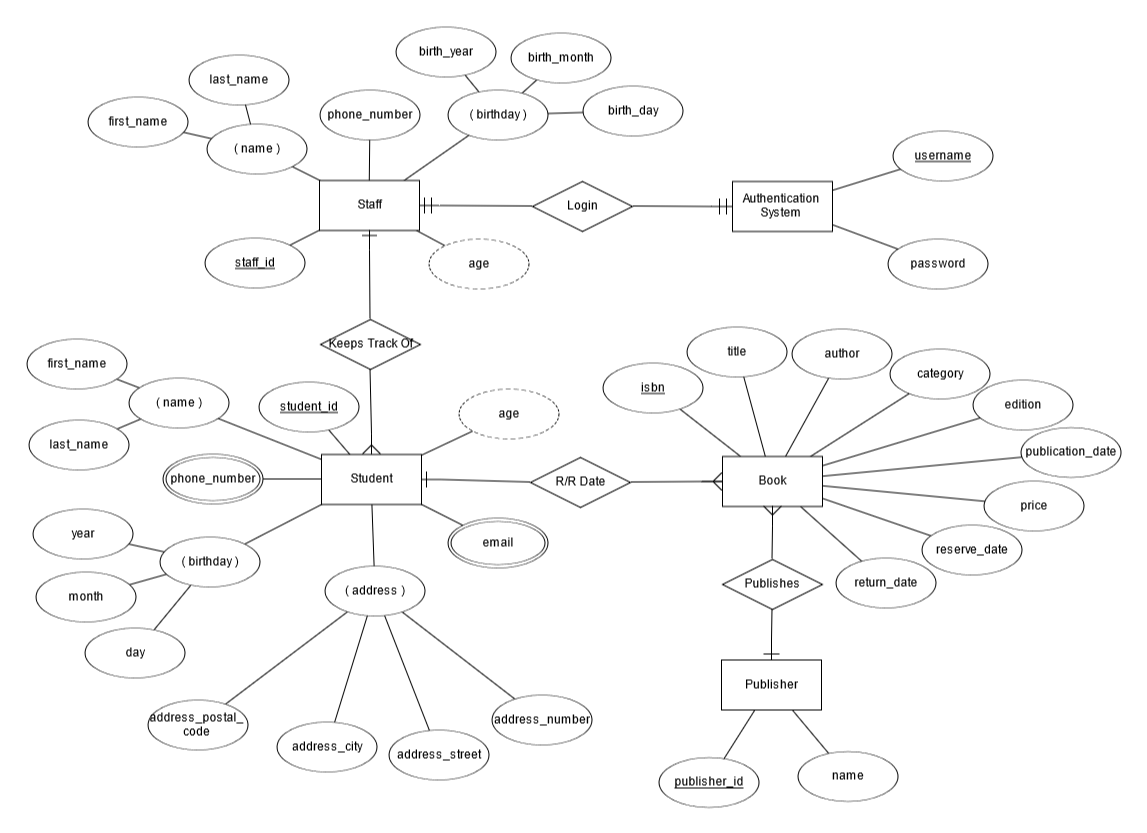
\includegraphics[width=\textwidth]{er_diagram.png}
		\end{center}
	
	\newpage
	\section{RS Diagram}
		\vspace{5cm}
		\begin{center}
			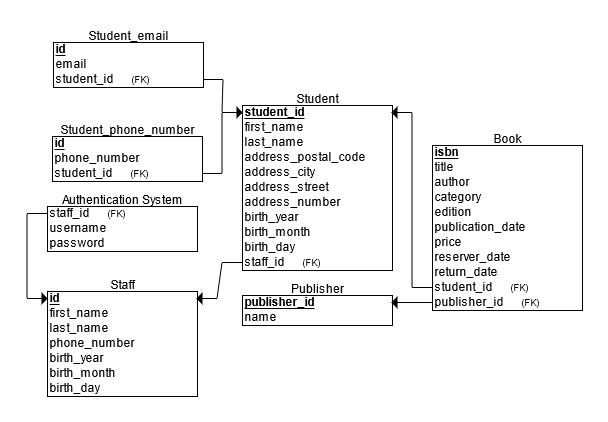
\includegraphics[width=\textwidth]{rs_diagram.png}
		\end{center}
		
	\newpage
	\section{SQL}
		The creation of the database was executed in Oracle.
		\subsection{Database Creation}
			\begin{verbatim}
CREATE TABLE Staff(
    id NUMBER(8,0) NOT NULL PRIMARY KEY,
    first_name VARCHAR(255) NOT NULL,
    last_name VARCHAR(255) NOT NULL,
    phone_number VARCHAR(255) NOT NULL,
    birth_year NUMBER(4,0) NOT NULL,
    birth_month NUMBER(2,0) NOT NULL,
    birth_day NUMBER(2,0) NOT NULL
);

CREATE TABLE Student(
    id NUMBER(8,0) NOT NULL PRIMARY KEY,
    first_name VARCHAR(255) NOT NULL,
    last_name VARCHAR(255) NOT NULL,
    address_postal_code VARCHAR(255) NOT NULL,
    address_city VARCHAR(255) NOT NULL,
    address_street VARCHAR(255) NOT NULL,
    address_number VARCHAR(255) NOT NULL,
    birth_year NUMBER(4,0) NOT NULL,
    birth_month NUMBER(2,0) NOT NULL,
    birth_day NUMBER(2,0) NOT NULL,
    staff_id NUMBER(8,0) NOT NULL,
    FOREIGN KEY (staff_id) REFERENCES Staff(id)
);

CREATE TABLE  Publisher(
    id NUMBER(1,0) NOT NULL PRIMARY KEY,
    name VARCHAR(255) NOT NULL
);
			\end{verbatim}
				
			\newpage
			\begin{verbatim}
CREATE TABLE Authentication_System(
    staff_id NUMBER(8,0) NOT NULL PRIMARY KEY,
    username VARCHAR(255) NOT NULL,
    password VARCHAR(255) NOT NULL,
    FOREIGN KEY(staff_id) REFERENCES Staff(id)
);

CREATE TABLE Student_email(
    id NUMBER(8,0) NOT NULL PRIMARY KEY,
    student_id NUMBER(8,0) NOT NULL,
    email VARCHAR(255),
    FOREIGN KEY(student_id) REFERENCES Student(id)
);

CREATE TABLE Student_phone_number(
    id NUMBER(8,0) NOT NULL PRIMARY KEY,
    student_id NUMBER(8,0) NOT NULL,
    phone_number VARCHAR(255) NOT NULL,
    FOREIGN KEY(student_id) REFERENCES Student(id)
);

CREATE TABLE Book(
    isbn VARCHAR(255) NOT NULL PRIMARY KEY,
    title VARCHAR(255) NOT NULL,
    author VARCHAR(255) NOT NULL,
    category VARCHAR(255) NOT NULL,
    edition VARCHAR(255) NOT NULL,
    publication_year NUMBER(4,0) NOT NULL,
    price INT NOT NULL,
    student_id NUMBER(8,0) NOT NULL,
    publisher_id NUMBER(1,0) NOT NULL,
    FOREIGN KEY(student_id) REFERENCES Student(id),
    FOREIGN KEY(publisher_id) REFERENCES Publisher(id)
);
			\end{verbatim}
			
		\newpage
		\subsection{Fill Database}
			I filled the tables with the INSERT command like this:\\
			\begin{center}
				INSERT INTO \textit{table} VALUES(\textit{id}, ...); 
			\end{center}
			Some examples from the staff database:
			\begin{center}
				INSERT INTO Staff VALUES(98017604, 'Axel', 'Nieri', '615-258-7302', 1968, 04, 16);\\
				INSERT INTO Staff VALUES(73267121, 'Red', 'Lowe', '715-993-3449', 1982, 04, 27);\\
				INSERT INTO Staff VALUES(26991745, 'Jelena', 'Kearney', '606-857-8284', 1953, 10, 01);\\
				INSERT INTO Staff VALUES(37065937, 'Jockel', 'Lu', '321-967-3130', 1979, 12, 30);\\
				INSERT INTO Staff VALUES(25187152, 'Sverrir', 'Gerhard', '303-892-6655', 1980, 11, 22);
			\end{center}
			The full list of commands used to fill up the database can found in the seperate .sql file.
		
		\subsection{Alter and Update Commands}
			Updates the wrong book title in the book table
			\begin{verbatim}
				UPDATE Book SET Book.title = 'Defender of dawn' WHERE Book.title = 'Fefender of dawn';
			\end{verbatim}		
			
			Update the wrong book category in the book table
			\begin{verbatim}
				UPDATE Book SET category='Adventure' WHERE category='Adcenture';
			\end{verbatim}
			
			Adds the non mandatory foundation date for each publisher
			\begin{verbatim}
				ALTER TABLE Publisher ADD founding_date date;
			\end{verbatim}						
		
		\subsection{Select Commands}
			
			Which students reserved the book titled: Game of wind?
			\begin{verbatim}
				SELECT Student.first_name, Student.last_name FROM Student JOIN Book
				ON Student.id = Book.student_id WHERE Book.title = 'Game of wind';
			\end{verbatim}
			
			How many students does each staff member handle?
			\begin{verbatim}
				SELECT Staff.id, COUNT(Student.id) FROM Staff JOIN Student
				ON Staff.id = Student.staff_id GROUP BY Staff.id;
			\end{verbatim}
				
			Distinct books in library and how many of each?
			\begin{verbatim}
				Select Book.title, COUNT(Book.title) FROM Book GROUP BY Book.title;
			\end{verbatim}
			
			Not reserved books.
			\begin{verbatim}
				Select Book.isbn, Book.title FROM Book WHERE Book.reserve_date IS NULL;
			\end{verbatim}
			
			
			\newpage
			How many books are resereved by each student.
			\begin{verbatim}
				SELECT Book.student_id, COUNT(*) "Number of Books" FROM Book GROUP BY Book.student_id;
			\end{verbatim}
			
			Number of books of each publisher.
			\begin{verbatim}
				SELECT Publisher.name, COUNT(Book.publisher_id) FROM Publisher JOIN Book
				ON Publisher.id = Book.publisher_id GROUP BY Publisher.name;
			\end{verbatim}
			
			Not reserved books with adventure category
			\begin{verbatim}
				SELECT Book.isbn, Book.title FROM Book WHERE
				Book.reserve_date IS NULL AND Book.category = 'Adventure';
			\end{verbatim}
			
			Students older than 18
			\begin{verbatim}
				SELECT Student.first_name, Student.last_name, Student.birth_year
				FROM Student WHERE Student.birth_year < 2004
			\end{verbatim}
\end{document}